\documentclass{svproc}

%\documentclass[a4paper, 10pt, conference]{ieeeconf}      % Use this line for a4 paper

\IEEEoverridecommandlockouts                              % This command is only needed if
                                                          % you want to use the \thanks command

\overrideIEEEmargins                                      % Needed to meet printer requirements.

%In case you encounter the following error:
%Error 1010 The PDF file may be corrupt (unable to open PDF file) OR
%Error 1000 An error occurred while parsing a contents stream. Unable to analyze the PDF file.
%This is a known problem with pdfLaTeX conversion filter. The file cannot be opened with acrobat reader
%Please use one of the alternatives below to circumvent this error by uncommenting one or the other
%\pdfobjcompresslevel=0
%\pdfminorversion=4

% See the \addtolength command later in the file to balance the column lengths
% on the last page of the document

% The following packages can be found on http:\\www.ctan.org
\usepackage{graphics} % for pdf, bitmapped graphics files
\usepackage{epsfig} % for postscript graphics files
\usepackage{mathptmx} % assumes new font selection scheme installed
\usepackage{times} % assumes new font selection scheme installed
\usepackage{amsmath} % assumes amsmath package installed
\usepackage{amssymb}  % assumes amsmath package installed
\usepackage{caption}
\usepackage{subcaption}
\usepackage{array}
\usepackage{siunitx}
\usepackage{tabularx}
\usepackage[T1]{fontenc}
\usepackage{makecell}
\usepackage{biblatex}
\bibliography{bibliography}

\title{\LARGE \bf
Laser Tracker Placement Optimization for highly flexible manufacturing systems
}



\author{Jan Baumgärtner$^{1*}$, Max Goebels$^{1*}$,   Alexander Puchta$^{1}$ and Jürgen Fleischer$^{1}$% <-this % stops a space
\thanks{*These authors contributed equally to this work.}% <-this % stops a space
\thanks{$^{1}$Jan Baumgärtner, Max Goebels, Alexander Puchta, and Jürgen Fleischer are with the wbk Institute of Production Science,
        Karlsruhe Institute of Technology, 76131 Karlsruhe, Germany
        {\tt\small max.goebels@kit.edu}}%
}



\begin{document}



\maketitle
\thispagestyle{empty}
\pagestyle{empty}


\section{Formulation of the optimization problem}
To solve the joint optimization problem of marker and laser tracker pose we first need to define the objective function.
Our goal is ofcourse to maximize the visibility of the marker to the laser tracker.
Similar to approaches such as~\cite{ieee_sensors} we divide the visibility into two components.
Line of sight visibility and field of view visibility.
Both  are depicted in figure~\ref{fig:visibility}.
\begin{figure}
        \centering
        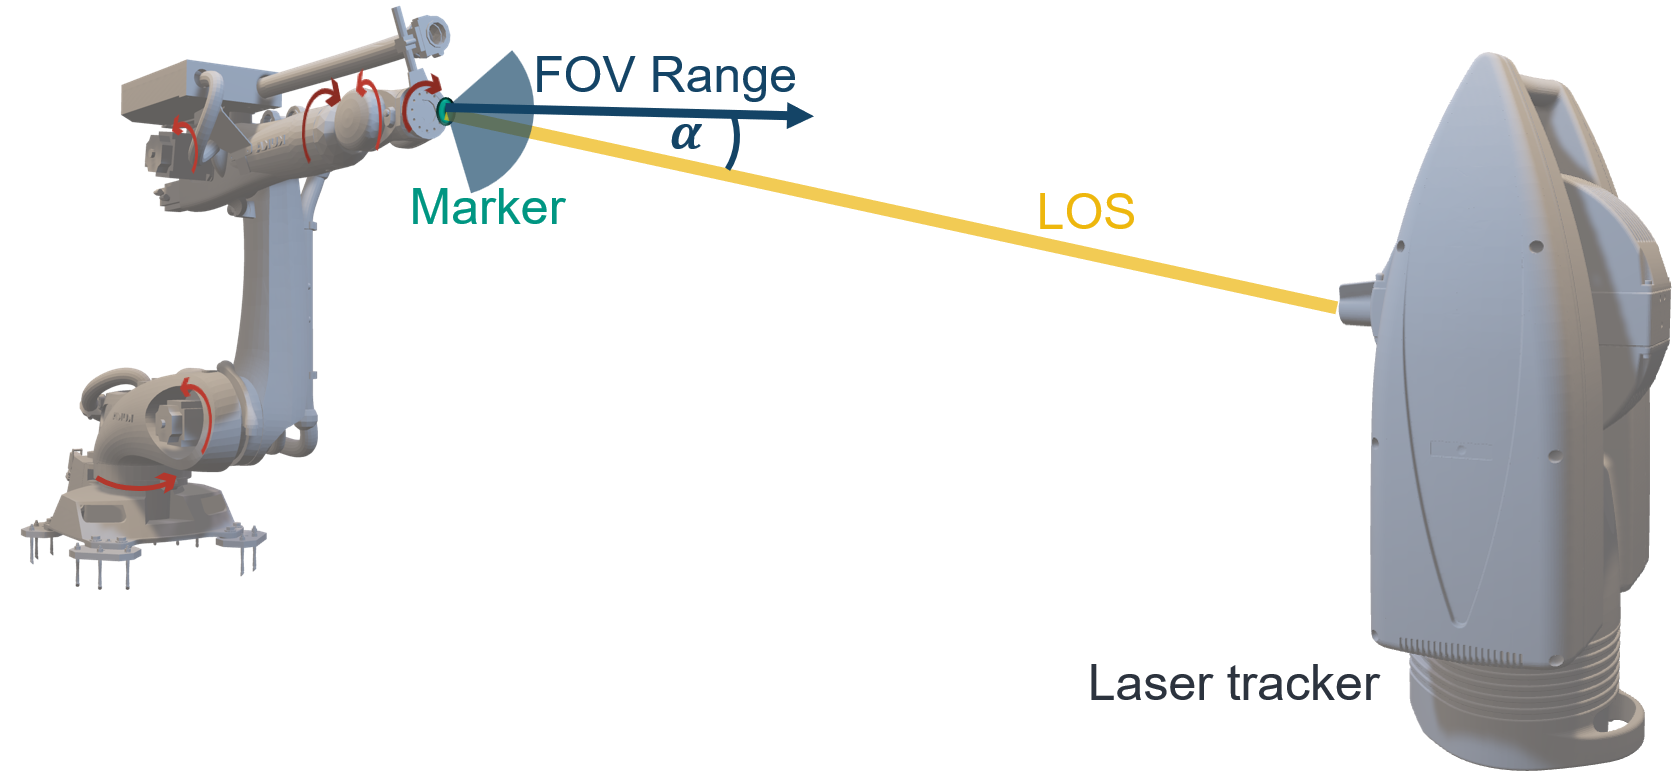
\includegraphics[width=0.8\textwidth]{figures/visibility.png}
        \caption{Field of view (VOW) angle range and line of sight (LOS) components of marker visibility}
        \label{fig:visibility}
\end{figure}
Mathematically we can define line of sight visibility (los visibility) as the following binary function:
\begin{equation}
    f(p_m,p_l) = \begin{cases}
    -1 & \text{if } \text{marker is in line of sight of the laser tracker} \\
    0 & \text{otherwise}
    \end{cases}
\end{equation}
where $p_m$ is the position of the marker, $p_l$ is the position of the laser tracker.
Note that $p_m$ is typically dependent on time as it is attached to a moving manufacuting system such as a robot.
The field of view objective can similarly be defined as a binary function:
\begin{equation}
    g(p_m,p_l) = \begin{cases}
    -1 & \text{if } \text{marker is in the field of view of the laser tracker} \\
    0 & \text{otherwise}
    \end{cases}
\end{equation}
However in practice it might make sense to not be close to the boundary of the field of view.
Instead one can define a continuous function that is 1 in the center of the field of view and 0 at the boundary.
The simplest way to encode this using the angle $\alpha$ between the normal of the marker and the line of sight of the laser tracker.
\begin{equation}
    g(p_m,p_l) = -\cos(\alpha)
\end{equation}
Apart from line of sight we also want to optimize the measurment performance of the laser tracker.
The accuracy of the lasertracker is mainly dependent on the distance between the marker and the laser tracker.
The further away the marker is the less accurate the measurment will be. However there is also a minimum measurment distance that the laser tracker can handle.
To encode this we can define a penalty function that penalizes markers that are too far away from the laser tracker.
\begin{equation}
    p(p_m,p_l) =  \begin{cases}
        d & \text{if marker is in measurement range of the laser tracker} \\
        \rho & \text{otherwise}
    \end{cases}
\end{equation}
where $d$ is the distance between the marker and the laser tracker, and $\rho$ is a large penalty factor.
The final objective function is then a weighted sum of the two components:
\begin{equation}
    h(p_m,p_l) = \int f(p_m,p_l) +  g(p_m,p_l) + p(p_m,p_l) \, dt
    \label{eq:objective}
\end{equation}

The intergral is taken over the entire trajectory of the manufacturing system that needs to be observed by the laser tracker.
Having defined the objective function, we can proceed to define the design variables and constraints.
The design variables are the pose of the laser tracker ($p_l$) and the pose of the marker ($p_m$).\\
\\
First, we assume the marker is attached to the flange of the manufacturing system, meaning we only need to define a transformation matrix $T_{m}$ that describes the marker's pose relative to the flange.
The final pose of the marker ($p_m$) is then given by combining the flange transformation $T_{f}(q)$, where $q$ is the robot's joint configuration, with the transformation $T_{m}$:

\begin{equation}
    p_m = T_{f}(q)T_{m}
\end{equation}

While $T_{m}$ is a 4x4 matrix, it can be parameterized using the marker's position ($p_{p_m}$) and orientation ($p_{o_m}$), resulting in a 6-dimensional design space for the marker pose.
To avoid unrealistic positions, we constrain this space to keep the marker close to the manufacturing system's surface.
This constraint can be represented cylindrically:
\begin{equation}
    \begin{split}
        \sqrt{p_{p_m,x}^2 + p_{p_m,y}^2} &\leq r \\
        0 \leq p_{p_m,z} &\leq h
    \end{split}
\end{equation}I

where $r$ is the cylinder's radius and $h$ is its height.
Additionally, to ensure the marker remains near the surface, a penalty function can be added to the objective function to penalize markers positioned too far from the flange.\\
\\
The laser tracker's pose is defined by a transformation matrix $T_{l}$, but due to its spherical measurement volume, only its position ($p_{p_l}$) needs to be specified.
The laser tracker is mounted on a stand with a height range constraint:
\begin{equation}
    h_{min} \leq p_{p_l,z} \leq h_{max}
\end{equation}
Where $h_{min}$ and $h_{max}$ are the minimum and maximum heights of the stand, respectively.
Using the design variables and constraints of the marker and laser tracker, the optimization problem can be formulated as follows:
\begin{equation}
    \begin{split}
        \max_{p_m,p_l} & \ h(p_m,p_l) \\
        \text{s.t.} & \ \sqrt{p_{p_m,x}^2 + p_{p_m,y}^2} \leq r \\
        & \ 0 \leq p_{p_m,z} \leq h \\
        & \ h_{min} \leq p_{p_l,z} \leq h_{max} \\
    \end{split}
\end{equation}


\section{Optimization algorithm}
There are a large number of possible optimization algorithms that can be used to solve this problem.
Following the no free lunch theorem we want to pick the algorithm that makes the most use of the underlying structure of the problem. %TODO citation needed
In this case the problem is a continuous optimization problem with a relatively low number of design variables.
On the other hand it is a gradient free optimization problem due to the line of sight visibility function.
These two properties make the problem well suited for the particle swarm optimization (pso) algorithm.
Particle swarm optimization (PSO) is a computational method for finding the optimal solution to a problem
 It is inspired by the behaviour of swarms in nature, such as flocks of birds or schools of fish, which exhibit emergent behaviour that is intelligent and efficient.
 In PSO, a group of particles (also called agents or individu-als) move through a search space, according to the fol-lowing update rules:
\begin{equation}
        \begin{split}
        x_{i,j} &= x_{i,j} + v_{i,j} \\
    v_{i,j} &= wv_{i,j} + c_1r_1(p_{i,j}-x_{i,j}) + c_2r_2(p_{g,j}-x_{i,j})
        \end{split}
\end{equation}
where $x_{i,j}$ is the position of particle $i$ in dimension $j$, $v_{i,j}$ is the velocity of particle $i$ in dimension $j$, $w$ is the inertia weight,
 $c_1$ and $c_2$ are the cognitive and social coefficients, $r_1$ and $r_2$ are random numbers between 0 and 1, $p_{i,j}$ is the best position of particle $i$ in dimension $j$ and $p_{g,j}$
is the best position of the swarm in dimension $j$.
In our case the particles are a 9 dimensional vector based on the position of the laser tracker and the pose of the marker.
The best particle is the one that maximizes the objective function defined in equation \ref{eq:objective}.
The hyperparameters we need to tune are collected in table \ref{tab:hyperparameters}.
Note that the pso algorithm has no direct way to encode the constraints we defined earlier.
Instead we can use a penalty function that penalizes any particles that violate the constraints.
This is a common approach in optimization and is also used in the implementation of the pso algorithm in the scipy library. %TODO citation needed
The penalty function can be defined as:
\begin{equation}
    p(x) =  \begin{cases}
        0 & \text{if } x \text{ satisfies all constraints} \\
        \rho & \text{otherwise}
    \end{cases}
\end{equation}
where $\rho$ is a large penalty factor.


\begin{table}  %TODO anpassen
        \centering
        \begin{tabular}{c|c}
                Hyperparameter & Value \\
                \hline
                Number of particles & 500 \\
                Number of iterations & 100 \\
                Inertia weight & 0.8 \\
                Cognitive coefficient & 0.1 \\
                Social coefficient & 0.1 \\
        \end{tabular}
        \caption{Hyperparameters of the PSO algorithm}
        \label{tab:hyperparameters}
\end{table}

\section{Simulation Environment}
Evaluating the objective function requires a simulation of the manufacturing system.
The tricky part here is that since the manufacturing is actively manufacturing parts we not only need to simulate the behavior of the system itself but the changing shape of any parts that are being manufactured.
For this purpose we are using the pybullet-industrial package \cite{pybullet_industrial}.
This extension of the pybullet physics engine allows us to simulate not only the robot but also the manufacturing process.
For the purposes of this paper the markers are implemented as a pybullet industrial endeffector obect that is attached to the robot.
A image of the simulation environment is shown in figure \ref{fig:simulation}.
\begin{figure}
        \centering
        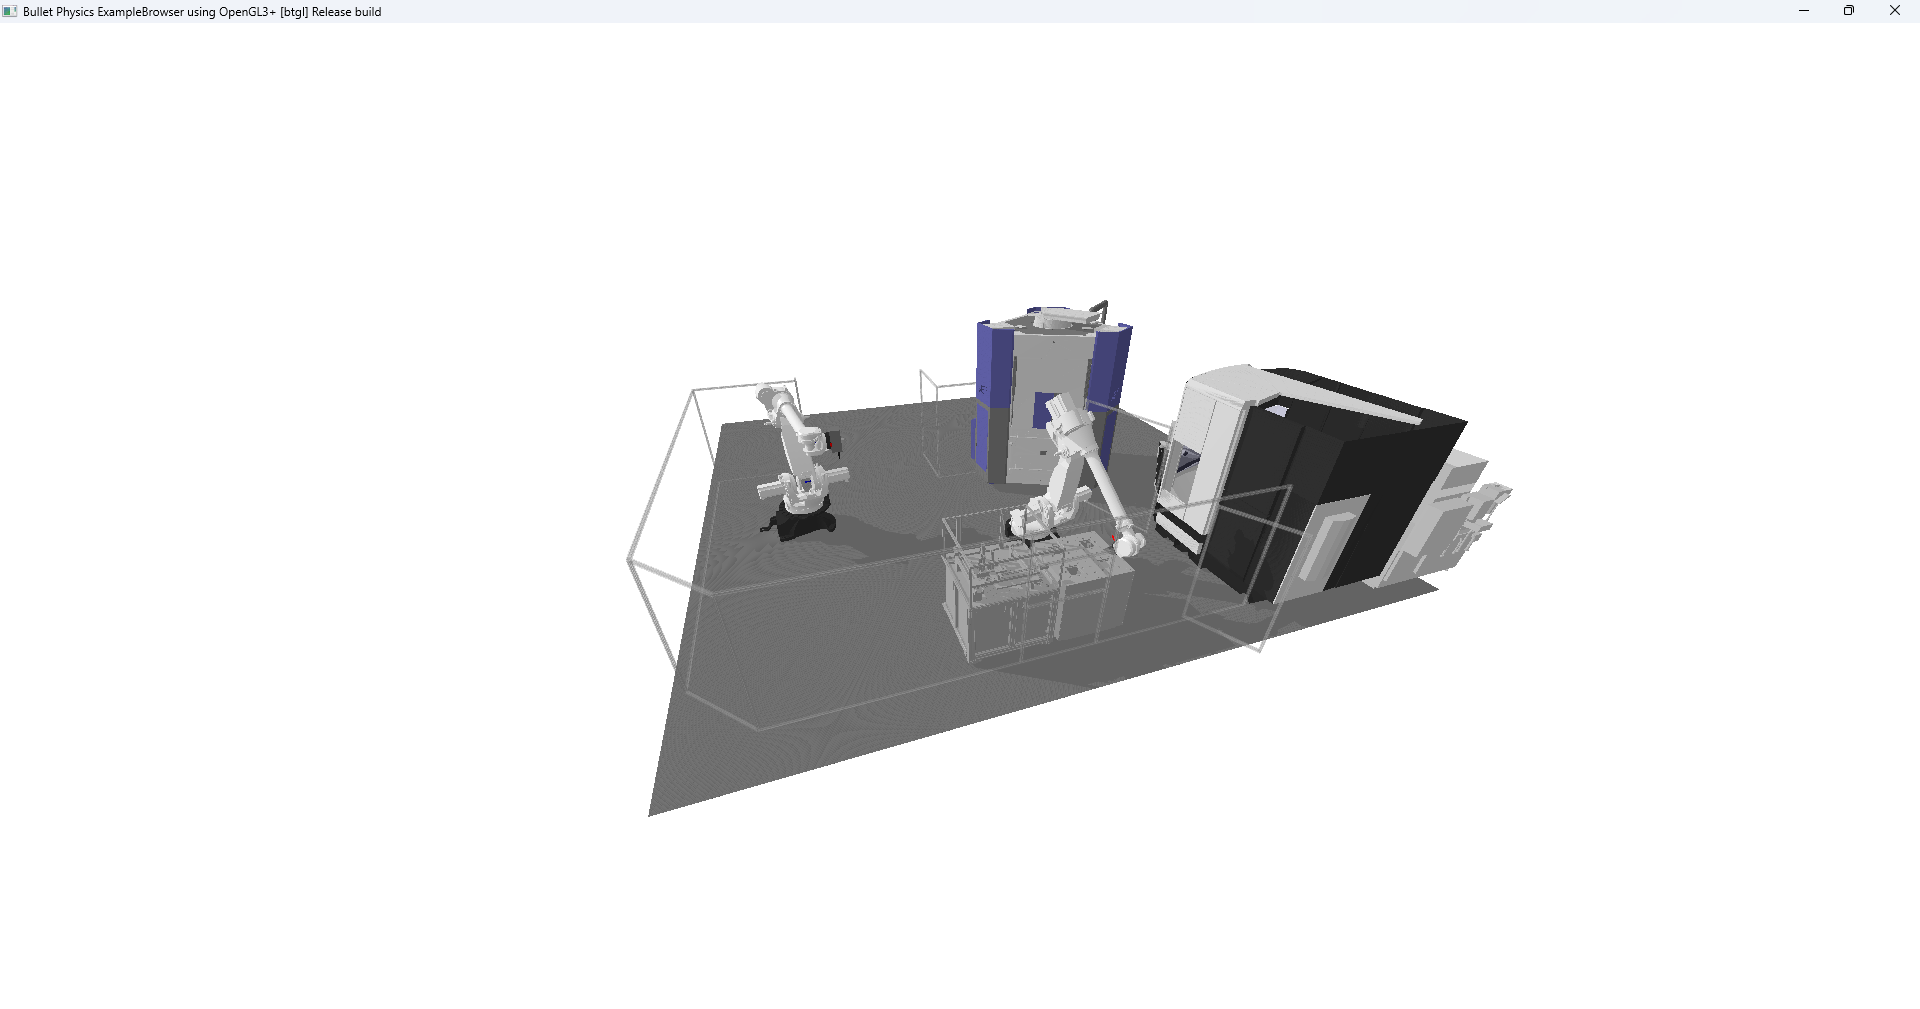
\includegraphics[width=\textwidth]{figures/simulation.png}
        \caption{Simulation environment used for the optimization}
        \label{fig:simulation}
\end{figure}

\section{Experiment Setup}
To test the performance of our optimizer, we need to define a testcase.
Both robots are Comau NJ290 industrial robots with a reach of 2.9 meters.
The right robot services the CNC machine and the additive manufacturing system, while the left robot performs a high-precision manufacturing task.
For this test, the left robot follows a rectangular trajectory with dimensions of 0.4 meters in length and 0.6 meters in width, as depicted in Figure \ref{fig:trajectory}.
The aim is now to find a laser tracker and marker placement that can track the left robot throughout its entire trajectory.
We compare this to the performance of the initial population of marker and laser tracker placements used to start the optimization process.
Figure \ref{fig:iterations} illustrates the performance of the algorithm over multiple iterations.
The results show that the algorithm converges to a solution in roughly 40 iterations, which is relatively fast for an optimization approach.
This speed is likely due to the existence of numerous optimal placements for the laser tracker and markers.
The final solution is also depicted in Figure \ref{fig:trajectory}.

\begin{figure}
\centering
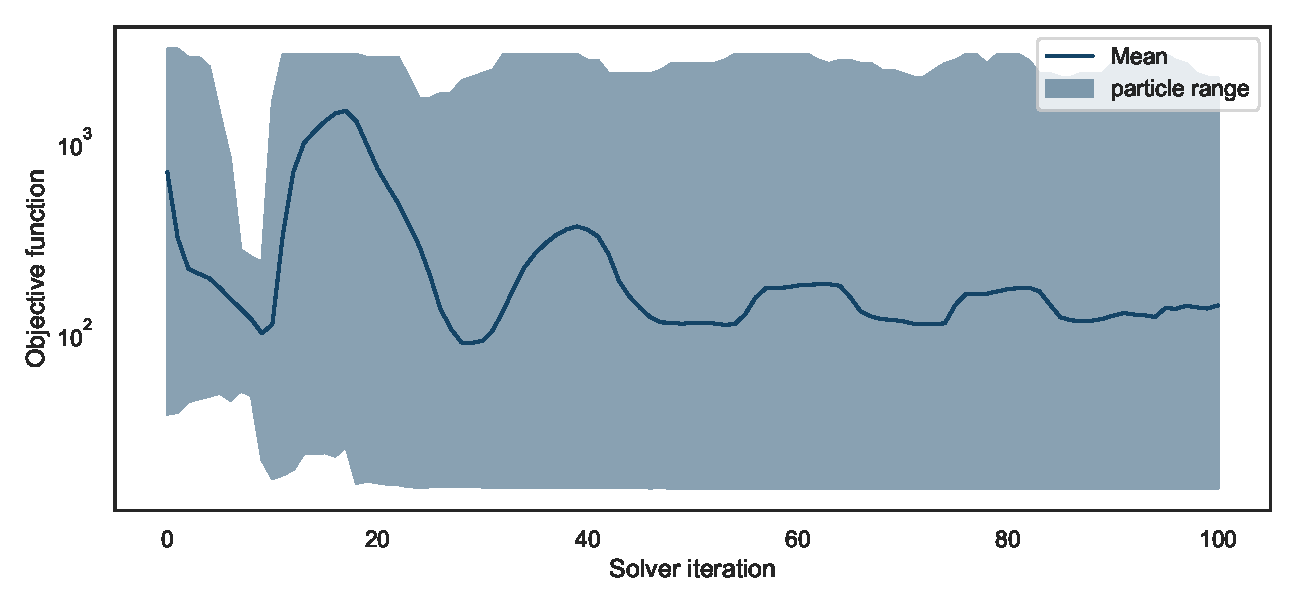
\includegraphics[width=\textwidth]{figures/iterations.pdf}
\caption{Performance of the algorithm over the iterations.}
\label{fig:iterations}
\end{figure}

\begin{figure}
\centering
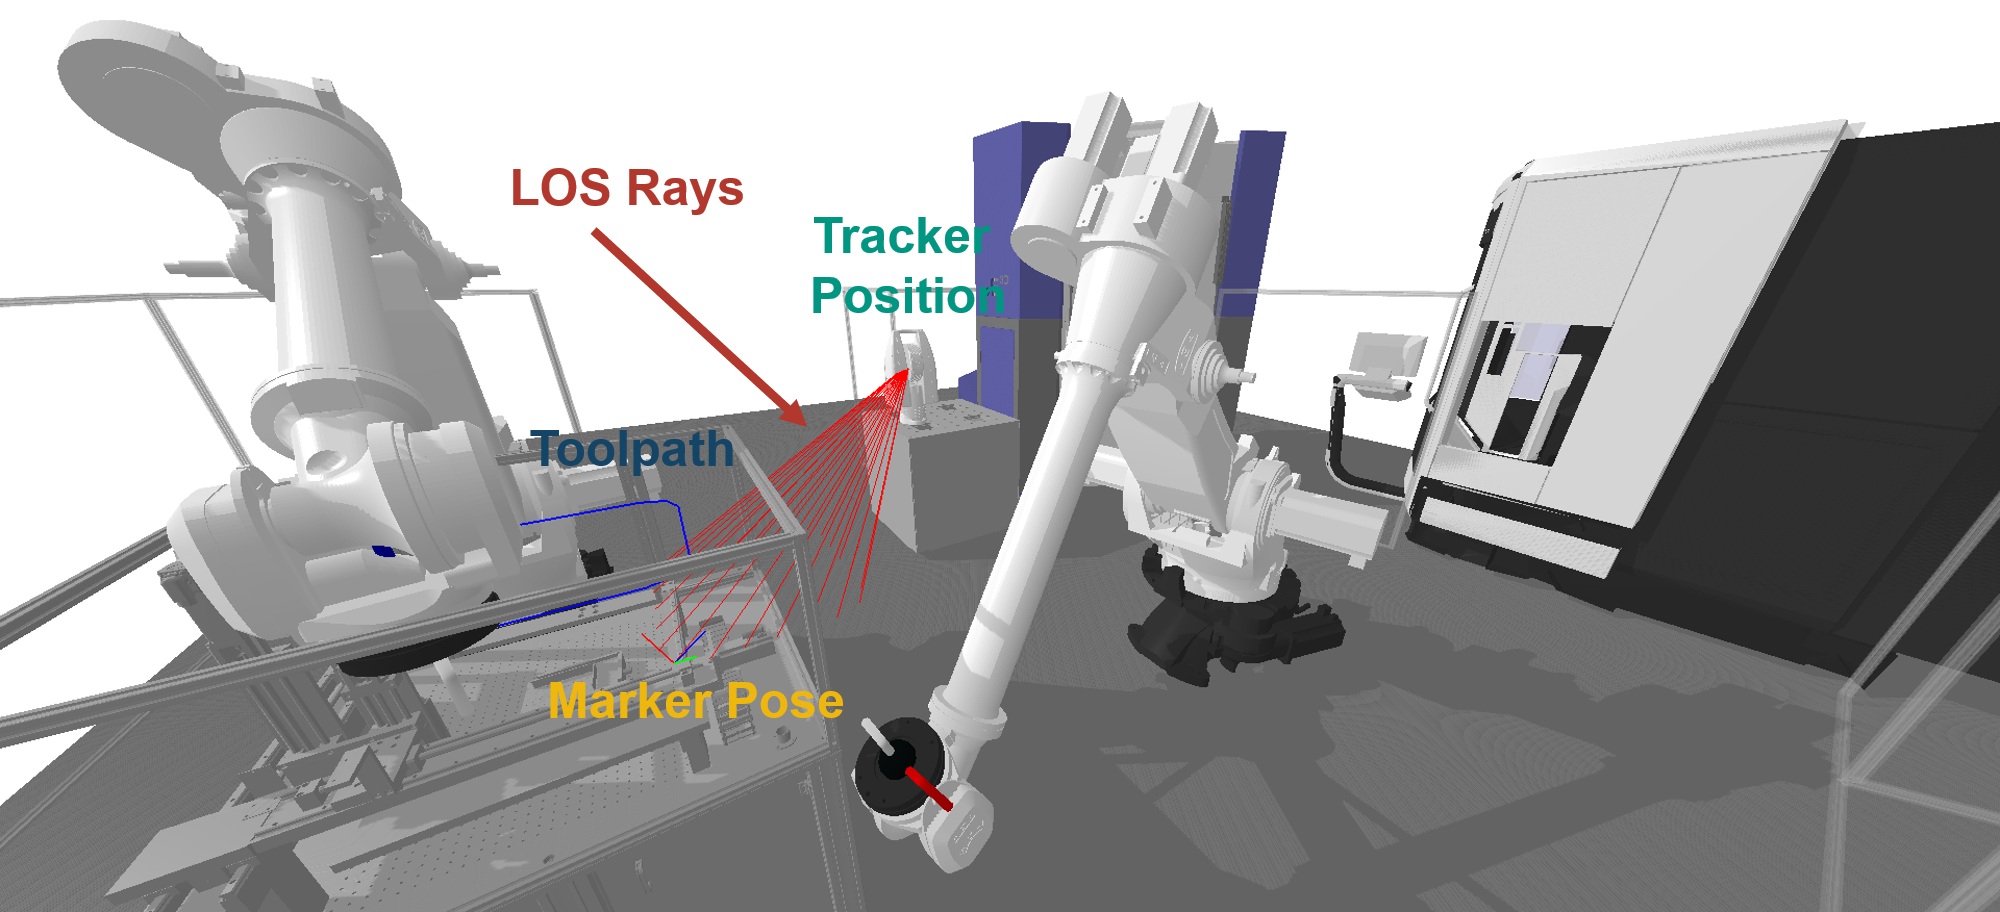
\includegraphics[width=0.8\textwidth]{figures/trajectory.png}
\caption{Trajectory of the robot and final laser tracker and marker placements.}
\label{fig:trajectory}
\end{figure}

\section{Acknowledgements}

%Bibliography
%TODO checken ob das stimmt in template
\printbibliography

\end{document}

